\documentclass[xetex,mathserif,serif]{beamer}
\usepackage{polyglossia}
\setdefaultlanguage[babelshorthands=true]{russian}
\usepackage{minted}
\usepackage{tabu}

\useoutertheme{infolines}

\usepackage{fontspec}
\setmainfont{FreeSans}
\newfontfamily{\russianfonttt}{FreeSans}

\definecolor{links}{HTML}{2A1B81}
\hypersetup{colorlinks,linkcolor=,urlcolor=links}

\tabulinesep=0.7mm

\newcommand{\attribution}[1] {
	\vspace{-5mm}\begin{flushright}\begin{scriptsize}\textcolor{gray}{\textcopyright\, #1}\end{scriptsize}\end{flushright}
}

\title{Обзор UML}
\author[Юрий Литвинов]{Юрий Литвинов \newline \textcolor{gray}{\small\texttt{yurii.litvinov@gmail.com}}}

\date{28.02.2019г}

\begin{document}
	
	\frame{\titlepage}

	\begin{frame}
		\frametitle{Unified Modeling Language}
		\begin{itemize}
			\item Семейство графических нотаций
			\begin{itemize}
				\item 14 видов диаграмм
			\end{itemize}
			\item Общая метамодель
			\item Стандарт под управлением Object Management Group
			\begin{itemize}
				\item UML 1.1 --- 1997 год
				\item UML 2.0 --- 2005 год
				\item UML 2.5.1 --- декабрь 2017 года
			\end{itemize}
			\item Прежде всего, для проектирования ПО
			\begin{itemize}
				\item После UML 2.0 стали появляться нотации и для инженеров
			\end{itemize}
			\item Расширяем
			\begin{itemize}
				\item Профили --- механизм легковесного расширения
				\item Метамоделирование
			\end{itemize}
		\end{itemize}
	\end{frame}

	\begin{frame}
		\frametitle{История}
		\begin{center}
			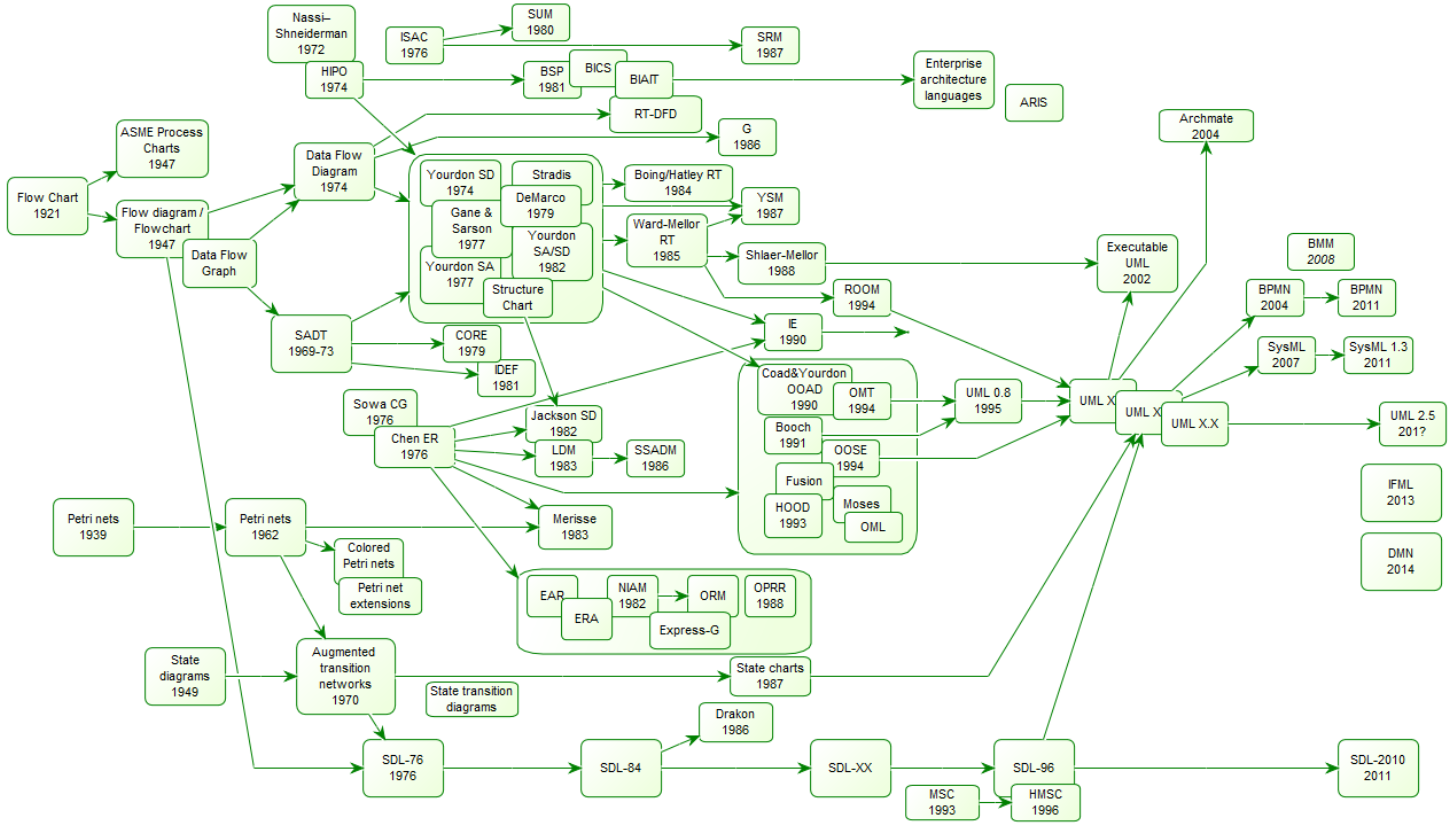
\includegraphics[width=\textwidth]{umlHistory.png}
		\end{center}
	\end{frame}

	\begin{frame}
		\frametitle{Виды диаграмм}
		\begin{center}
			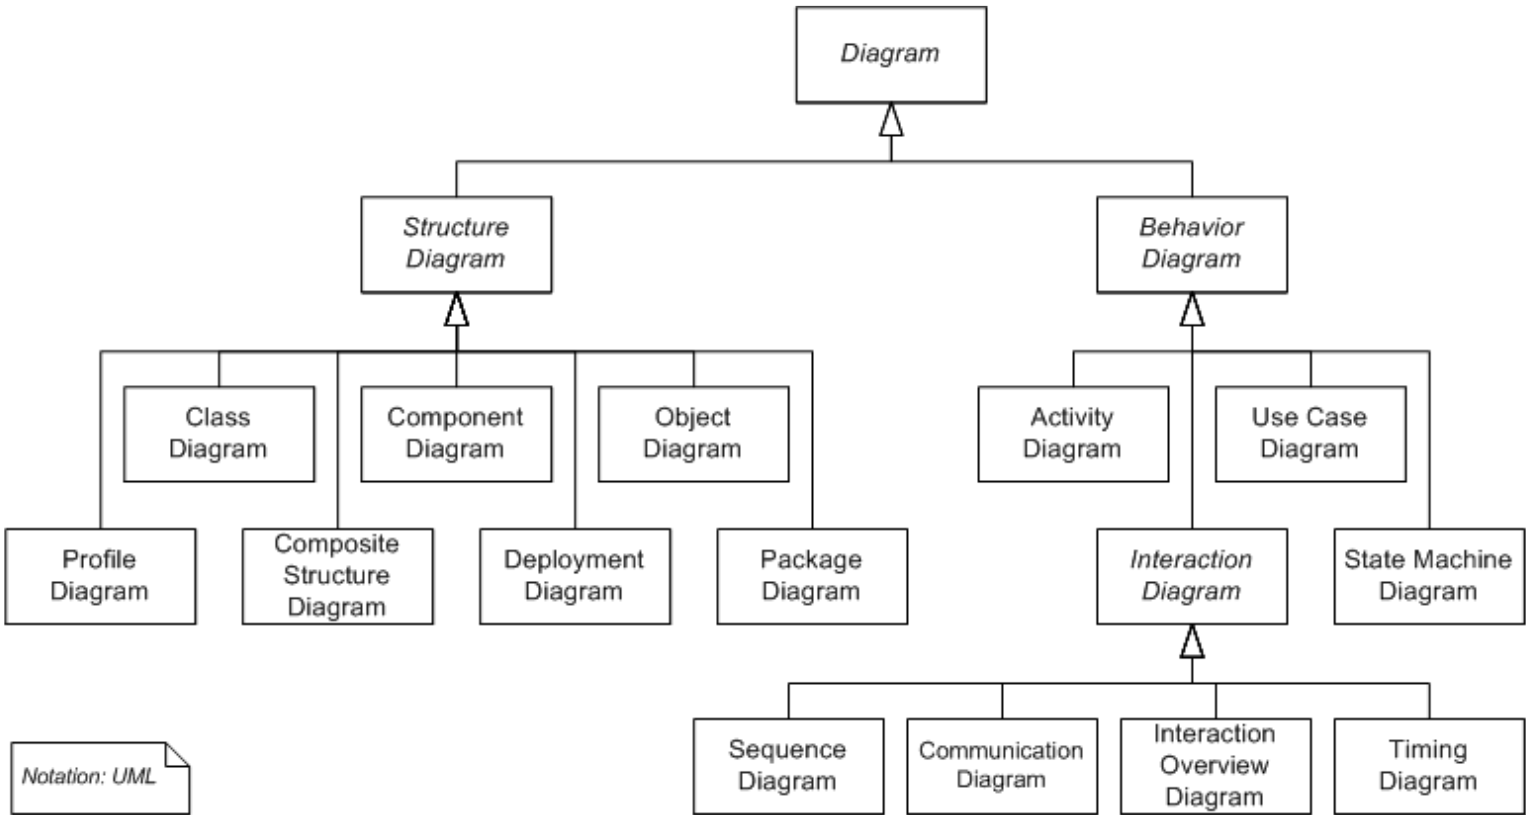
\includegraphics[width=\textwidth]{umlDiagrams.png}
		\end{center}
	\end{frame}

	\section{Диаграмма классов UML}

	\begin{frame}
		\frametitle{Диаграмма классов}
		\begin{center}
			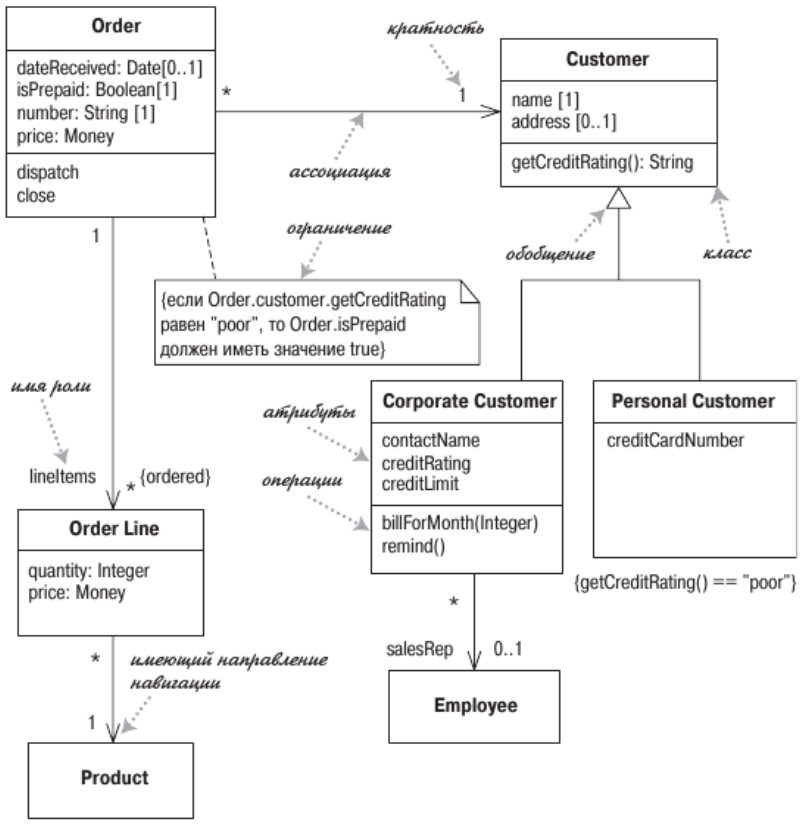
\includegraphics[height=0.8\textheight]{umlClassDiagram.png}
			\attribution{М. Фаулер. ``UML. Основы''}
		\end{center}
	\end{frame}

	\section{Диаграммы пакетов}

	\begin{frame}
		\frametitle{Диаграммы пакетов}
		\begin{center}
			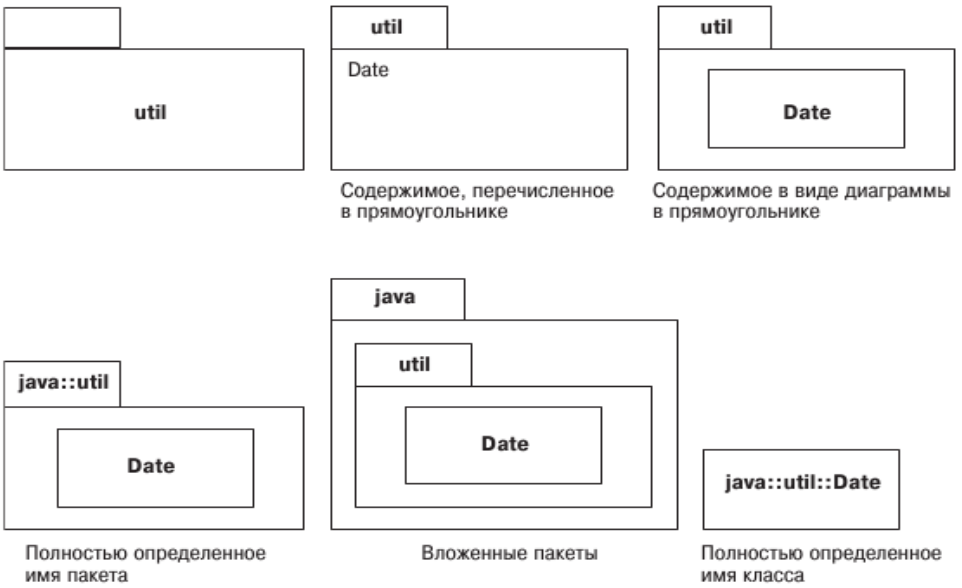
\includegraphics[width=0.8\textwidth]{packageDiagrams.png}
			\attribution{М. Фаулер. ``UML. Основы''}
		\end{center}
	\end{frame}

	\begin{frame}
		\frametitle{Диаграммы пакетов, зависимости}
		\begin{center}
			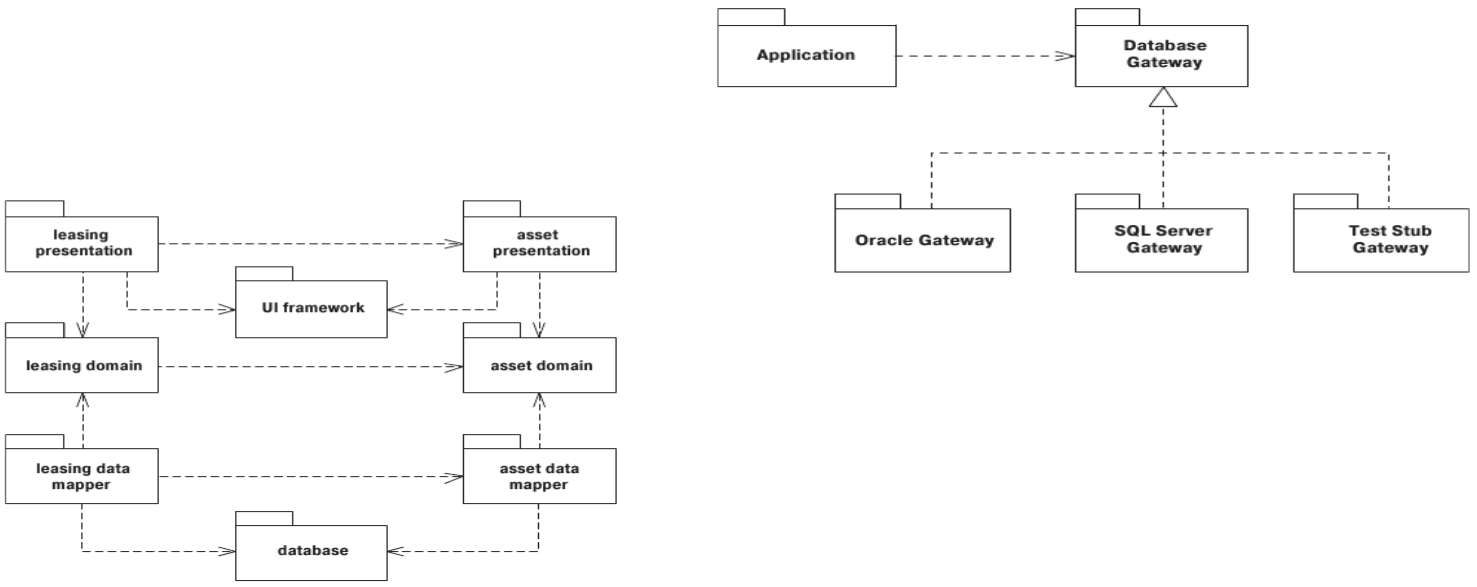
\includegraphics[width=0.95\textwidth]{packageDependencies.png}
			\attribution{М. Фаулер. ``UML. Основы''}
		\end{center}
	\end{frame}

	\section{Диаграммы объектов}

	\begin{frame}
		\frametitle{Диаграммы объектов}
		\begin{center}
			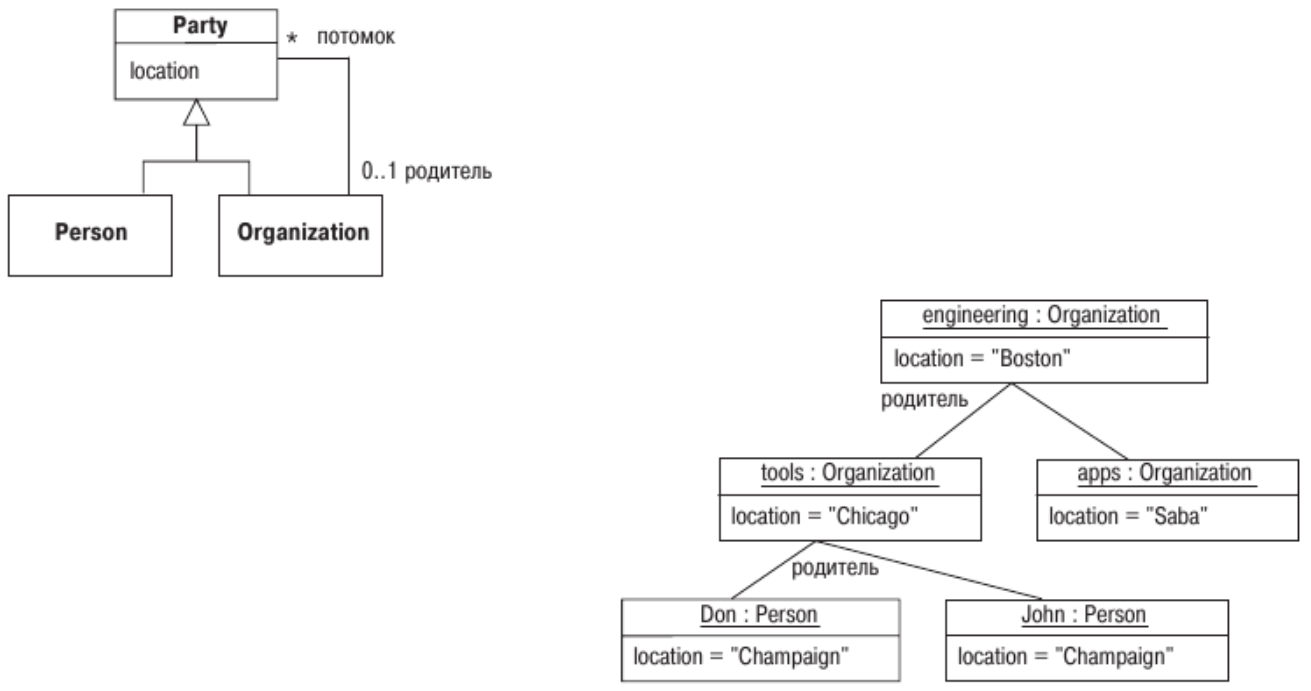
\includegraphics[width=0.9\textwidth]{objectDiagrams.png}
			\attribution{М. Фаулер. ``UML. Основы''}
		\end{center}
	\end{frame}

	\section{Диаграммы компонентов}
	
	\begin{frame}
		\frametitle{Диаграммы компонентов}
		\begin{center}
			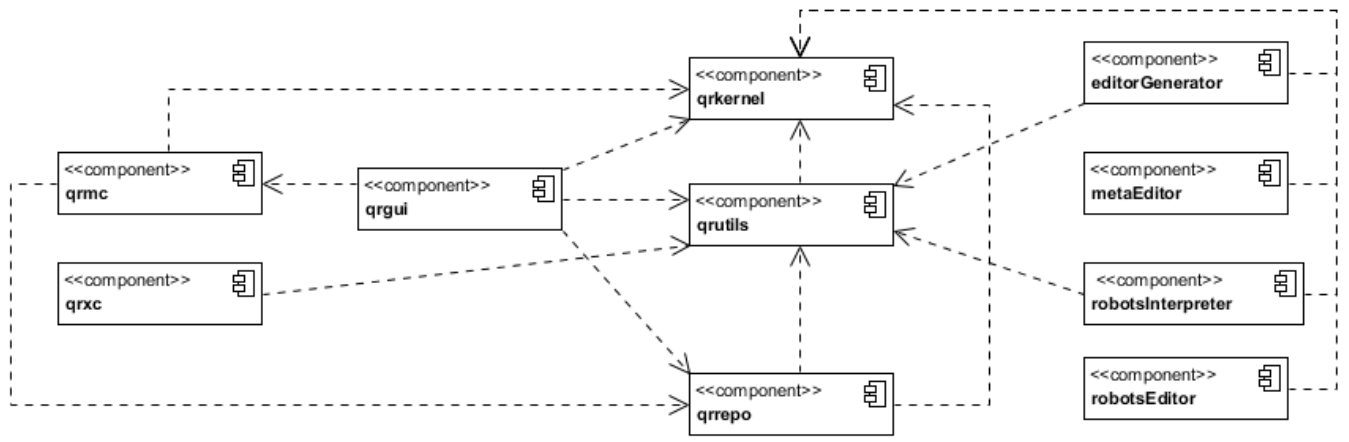
\includegraphics[width=0.95\textwidth]{componentDiagrams.png}
		\end{center}
	\end{frame}

	\begin{frame}
		\frametitle{Более подробно}
		\begin{center}
			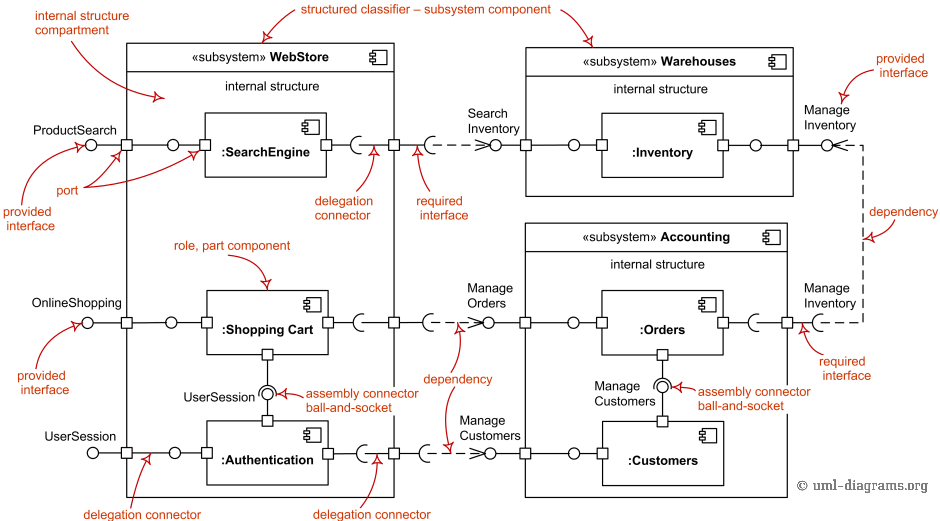
\includegraphics[width=0.95\textwidth]{componentDiagramsOverview.png}
			\attribution{\url{http://www.uml-diagrams.org}}
		\end{center}
	\end{frame}

	\section{Моделирование случаев использования}
	
	\begin{frame}
		\frametitle{Диаграмма случаев использования UML}
		\framesubtitle{Диаграмма прецедентов}
		\begin{columns}
			\begin{column}{0.5\textwidth}
				\begin{itemize}
					\item Ивар Якобсон, 1992 год
					\item Акторы (или актёры, роли) --- внешние сущности, использующие систему
					\begin{itemize}
						\item Люди или другие программные системы
					\end{itemize}
					\item Случаи использования (прецеденты)  --- цель использования системы актором
					\begin{itemize}
						\item Раскрываются в набор сценариев, описываемых чаще текстом
					\end{itemize}
				\end{itemize}
			\end{column}
			\begin{column}{0.5\textwidth}
				\begin{center}
					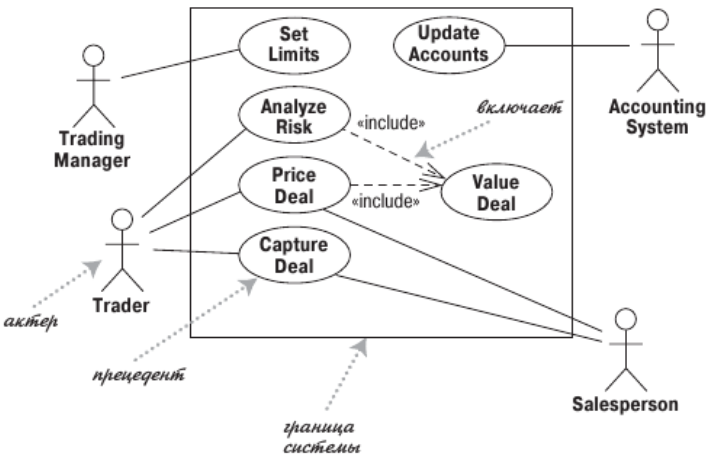
\includegraphics[width=\textwidth]{useCaseDiagram.png}
					\attribution{М. Фаулер, UML. Основы}
				\end{center}
			\end{column}
		\end{columns}
	\end{frame}

	\begin{frame}
		\frametitle{Пример, check-in в аэропорту}
		\begin{center}
			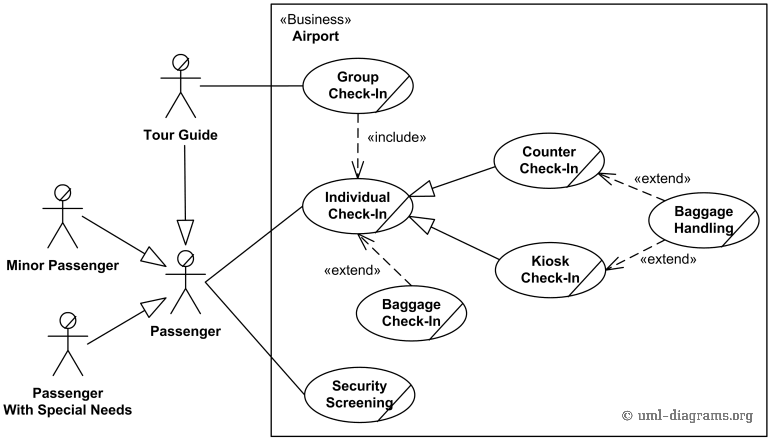
\includegraphics[width=0.7\textwidth]{airportUseCase.png}
			\attribution{http://www.uml-diagrams.org}
		\end{center}
	\end{frame}

	\begin{frame}
		\frametitle{Случай использования, типичная структура}
		\begin{itemize}
			\item Заголовок (цель основного актора)
			\item Заинтересованые лица, акторы, основной актор
			\item Предусловия
			\item Триггеры (активаторы)
			\item Основной порядок событий
			\item Альтернативные пути и расширения
			\item Постусловия
		\end{itemize}
	\end{frame}

	\begin{frame}
		\begin{center}
			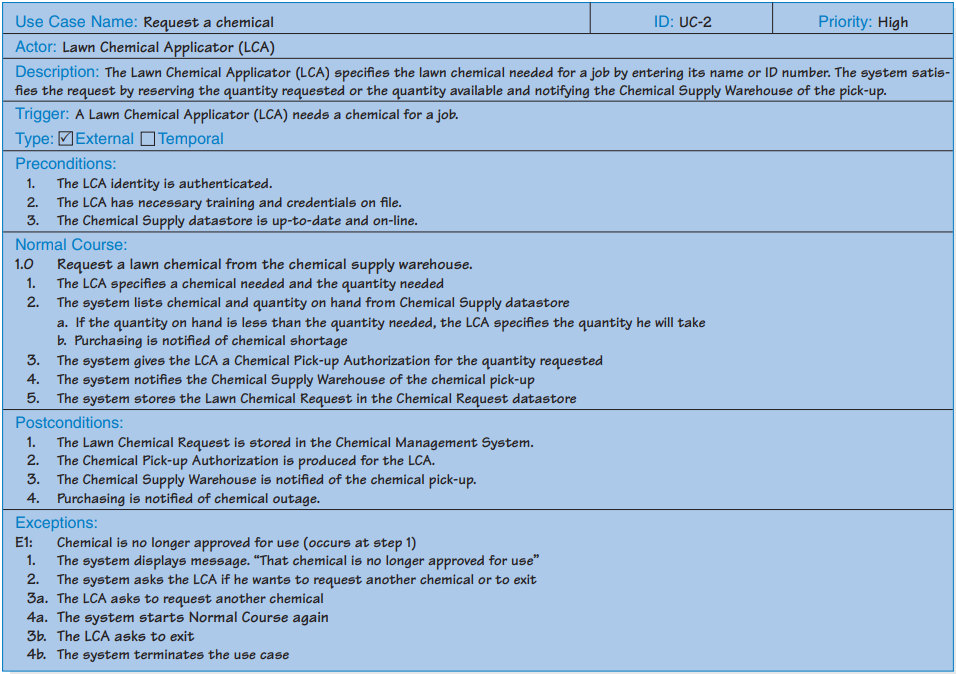
\includegraphics[width=0.9\textwidth]{useCaseExample.png}
			\attribution{R.M. Roth et al., System Analysis and Design}
		\end{center}
	\end{frame}

	\section{Диаграмма активностей UML}

	\begin{frame}
		\frametitle{Диаграмма активностей UML}
		\framesubtitle{Диаграммы деятельности}
		\begin{columns}
			\begin{column}{0.5\textwidth}
				\begin{itemize}
					\item Используются для моделирования бизнес-процессов, тоже на первых этапах
					\begin{itemize}
						\item Может быть визуализацией сценария использования
					\end{itemize}
					\item Иногда --- для моделирования алгоритма
					\item Расширенные блок-схемы
					\item Семантика на основе сетей Петри
				\end{itemize}
			\end{column}
			\begin{column}{0.5\textwidth}
				\begin{center}
					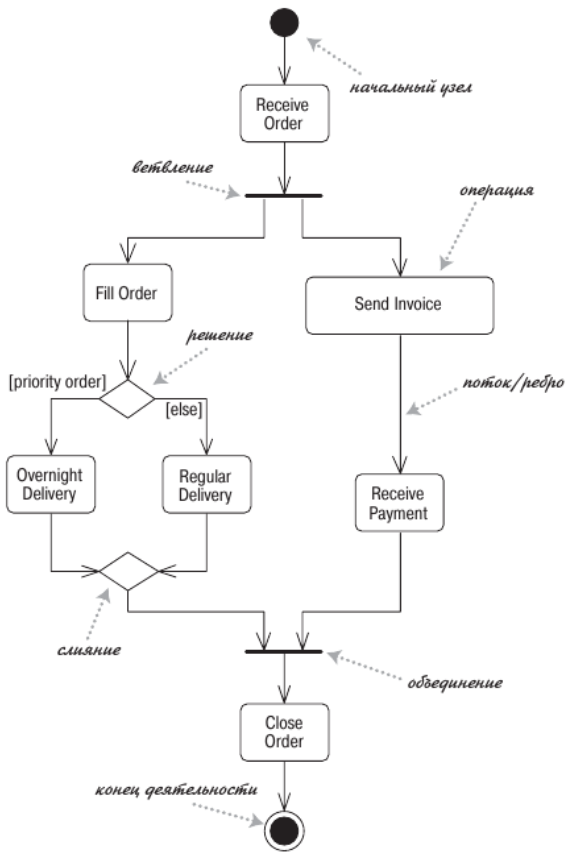
\includegraphics[width=0.7\textwidth]{activityDiagram.png}
					\attribution{М. Фаулер, UML. Основы}
				\end{center}
			\end{column}
		\end{columns}
	\end{frame}

	\begin{frame}
		\frametitle{Диаграмма активностей, разделы}
		\begin{columns}
			\begin{column}{0.5\textwidth}
				\begin{itemize}
					\item Раздел представляет отдел организации (или организацию), отвечающий за часть работы
					\item Визуализирует поток работ между отделами
				\end{itemize}
			\end{column}
			\begin{column}{0.5\textwidth}
				\begin{center}
					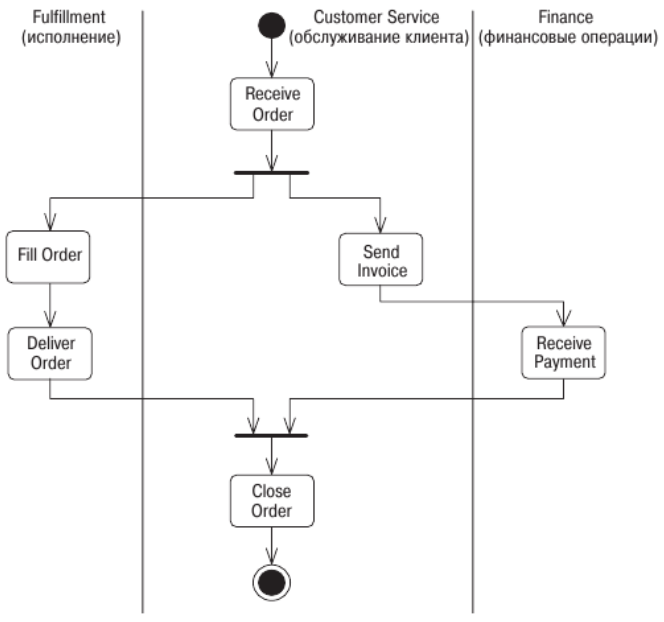
\includegraphics[width=0.9\textwidth]{activitySwimlanes.png}
					\attribution{М. Фаулер, UML. Основы}
				\end{center}
			\end{column}
		\end{columns}
	\end{frame}

	\begin{frame}
		\frametitle{Диаграмма активностей, сигналы}
		\begin{itemize}
			\item Для визуализации асинхронных процессов
			\item Сигналом может быть посылка документа, запрос и т.д.
		\end{itemize}
		\begin{center}
			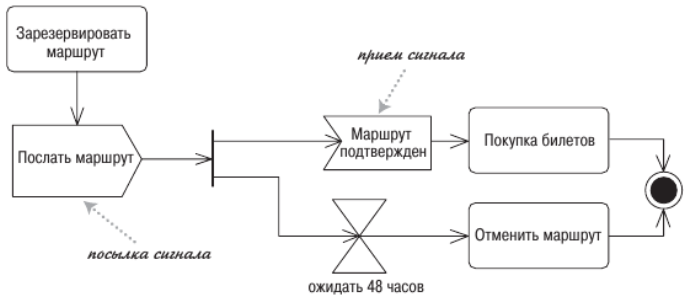
\includegraphics[width=0.6\textwidth]{activitySignals.png}
			\attribution{М. Фаулер, UML. Основы}
		\end{center}
	\end{frame}

	\section{Диаграмма развёртывания}
	
	\begin{frame}
		\frametitle{Диаграмма развёртывания UML}
		\begin{columns}
			\begin{column}{0.5\textwidth}
				\begin{itemize}
					\item Показывает отображение компонентов и физических артефактов на реальные (или виртуальные) устройства
					\item Бывает полезна на начальных этапах проектирования, даже до диаграмм компонентов
				\end{itemize}
			\end{column}
			\begin{column}{0.5\textwidth}
				\begin{center}
					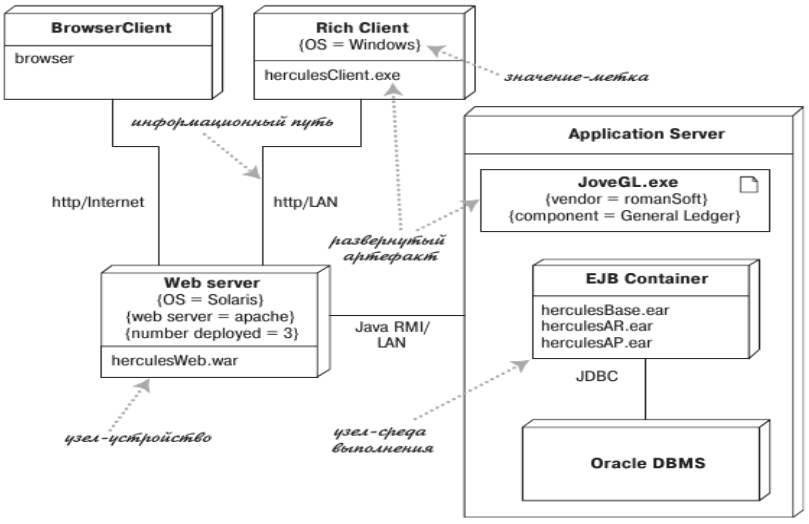
\includegraphics[width=\textwidth]{deploymentDiagram.png}
					\attribution{М. Фаулер, UML. Основы}
				\end{center}
			\end{column}
		\end{columns}
	\end{frame}

	\section{Диаграммы состояний}

	\begin{frame}
		\frametitle{Диаграммы конечных автоматов}
		\framesubtitle{Диаграммы состояний}
		\begin{columns}
			\begin{column}{0.5\textwidth}
				\begin{itemize}
					\item Состояния объекта как часть жизненного цикла
					\item Моделирование реактивных объектов
					\begin{itemize}
						\item Например, сетевое соединение
						\item Или знакомый пример с торговым автоматом
					\end{itemize}
					\item Имеют исполнимую семантику
					\item Д. Харел, 1987
				\end{itemize}
			\end{column}
			\begin{column}{0.5\textwidth}
				\begin{center}
					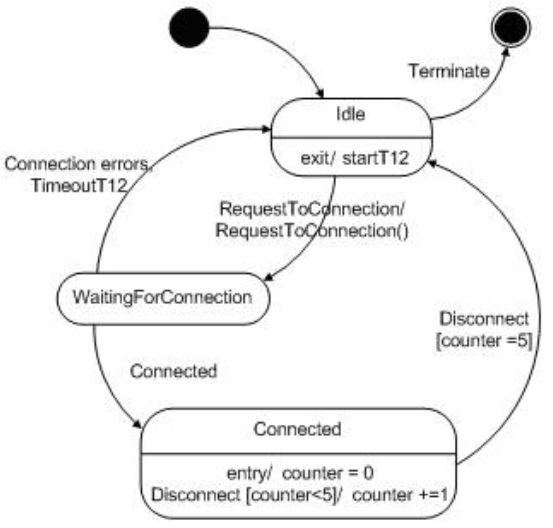
\includegraphics[width=0.7\textwidth]{stateTransitionExample.png}
				\end{center}
			\end{column}
		\end{columns}
	\end{frame}

	\begin{frame}
		\frametitle{Диаграммы конечных автоматов, синтаксис}
		\begin{columns}
			\begin{column}{0.5\textwidth}
				\begin{itemize}
					\item Состояние
					\begin{itemize}
						\item entry activity
						\item exit activity
						\item do activity
						\item внутренний переход
					\end{itemize}
					\item Событие
					\item Переход
					\begin{itemize}
						\item имя события (список параметров) [сторожевое условие] выражение действия
					\end{itemize}
				\end{itemize}
			\end{column}
			\begin{column}{0.5\textwidth}
				\begin{center}
					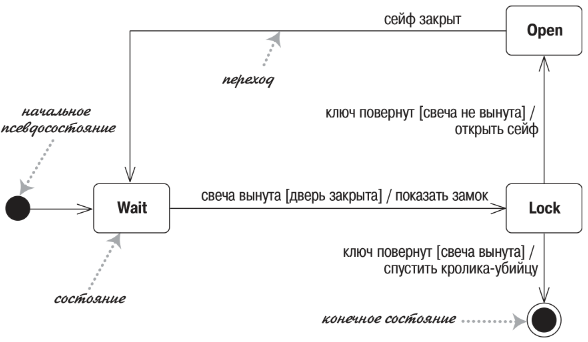
\includegraphics[width=\textwidth]{stateTransitionSyntax.png}
					\attribution{М. Фаулер, UML. Основы}
				\end{center}
			\end{column}
		\end{columns}
	\end{frame}

	\begin{frame}
		\frametitle{Пример, мобильный телефон}
		\begin{center}
			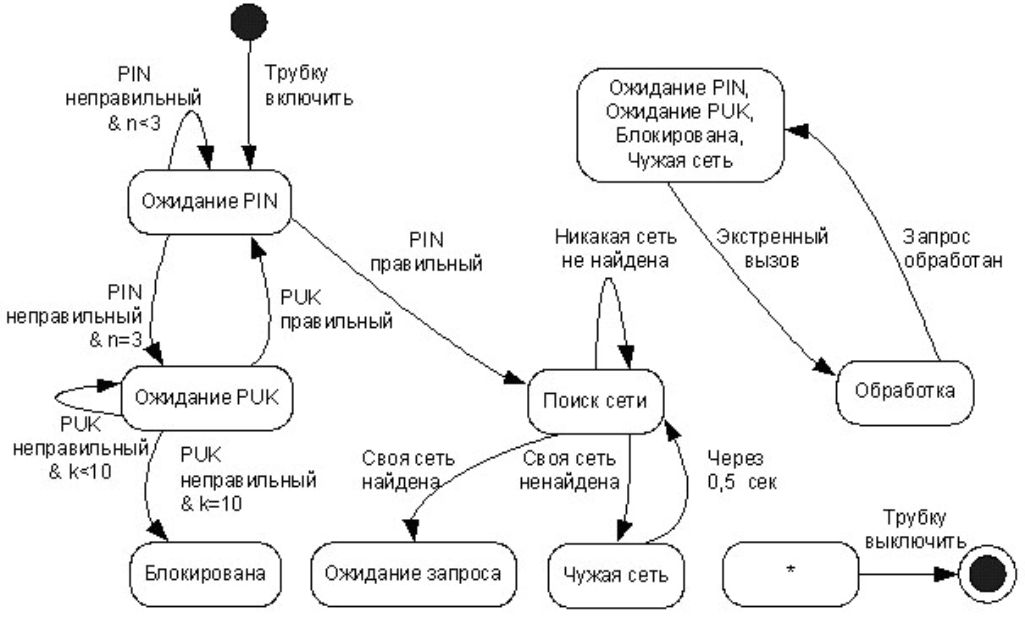
\includegraphics[width=0.7\textwidth]{stateTransitionExample2.png}
		\end{center}
	\end{frame}

	\begin{frame}
		\frametitle{Диаграммы конечных автоматов, прочие вещи}
		Активности:
		\begin{columns}
			\begin{column}{0.5\textwidth}
				\begin{center}
					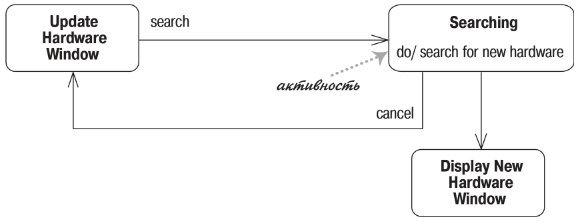
\includegraphics[width=\textwidth]{stateTransitionInternalEventExample.png}
				\end{center}
			\end{column}
			\begin{column}{0.5\textwidth}
				\begin{center}
					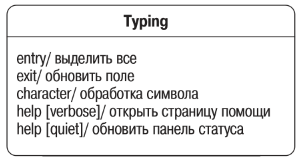
\includegraphics[width=0.5\textwidth]{stateTransitionInternalEvents.png}
				\end{center}
			\end{column}
		\end{columns}

		\begin{columns}
			\begin{column}{0.5\textwidth}
				Вложенные состояния:
				\begin{center}
					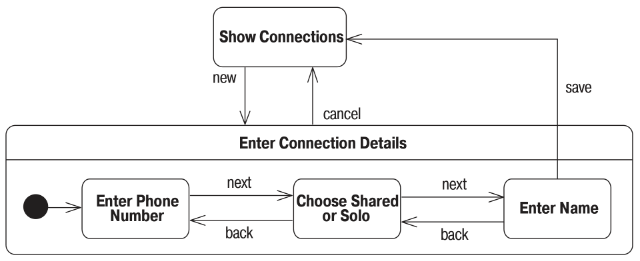
\includegraphics[width=\textwidth]{stateTransitionNestedStates.png}
					\attribution{М. Фаулер, UML. Основы}
				\end{center}
			\end{column}
			\begin{column}{0.5\textwidth}
				Параллельные состояния, псевдосостояние истории:
				\begin{center}
					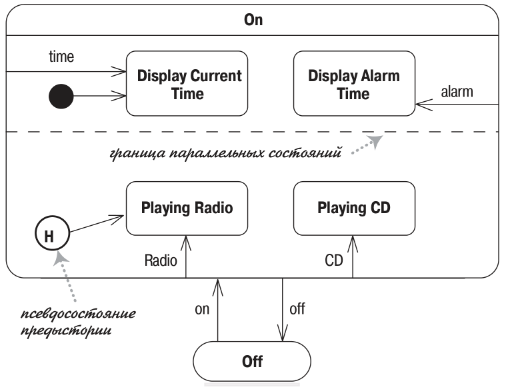
\includegraphics[width=0.7\textwidth]{stateTransitionParallelStates.png}
				\end{center}
			\end{column}
		\end{columns}
	\end{frame}

	\begin{frame}[fragile]
		\frametitle{Генерация кода}
		\begin{columns}
			\begin{column}{0.5\textwidth}
				\begin{tiny}
					\begin{minted}{java}
public void handleEvent(PanelEvent anEvent) {
    switch (currentState) {
        case PanelState.Open:
            switch (anEvent) {
                case PanelEvent.SafeClosed:
                    currentState = PanelState.Wait;
            }
            break;
        case PanelState.Wait:
            switch (anEvent) {
                case PanelEvent.CandleRemoved:
                    if (isDoorOpen) {
                        revealLock();
                        currentState = PanelState.Lock;
                    }
            }
            break;
        case PanelState.Lock:
            switch (anEvent) {
                case PanelEvent.KeyTurned:
                    if (isCandleIn) {
                        openSafe();
                        currentState = PanelState.Open;
                    } else {
                        releaseKillerRabbit();
                        currentState = PanelState.Final;
                    }
            }
            break;
    }
}
					\end{minted}
				\end{tiny}
			\end{column}
			\begin{column}{0.5\textwidth}
				\begin{center}
					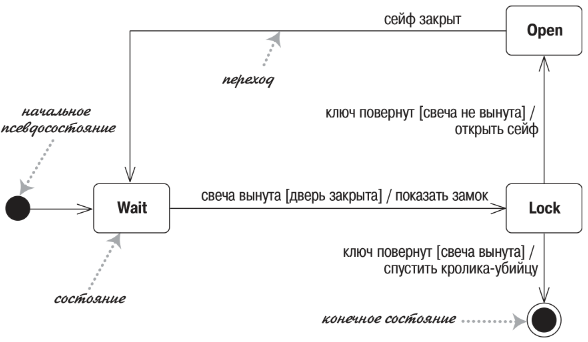
\includegraphics[width=\textwidth]{stateTransitionSyntax.png}
					\attribution{М. Фаулер, UML. Основы}
				\end{center}
			\end{column}
		\end{columns}
	\end{frame}

	\begin{frame}
		\frametitle{Таблица состояний}
		\begin{center}
			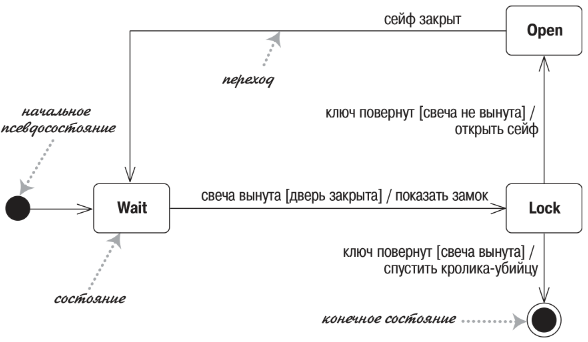
\includegraphics[width=0.4\textwidth]{stateTransitionSyntax.png}
		\end{center}

		\begin{center}
			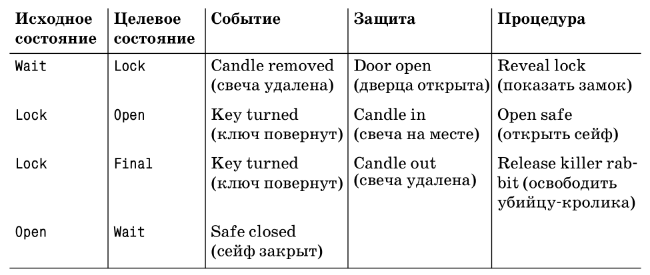
\includegraphics[width=0.5\textwidth]{stateTransitionStateTable.png}
			\attribution{М. Фаулер, UML. Основы}
		\end{center}
	\end{frame}

	\begin{frame}
		\frametitle{Паттерн ``Состояние''}
		\begin{center}
			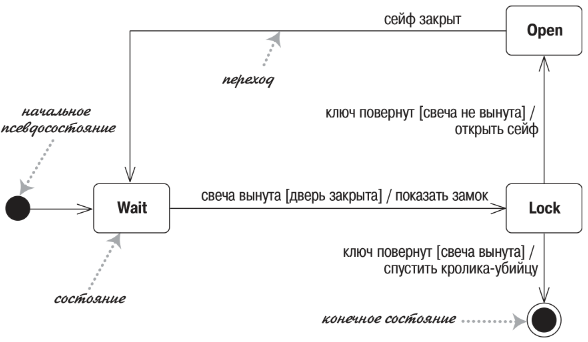
\includegraphics[width=0.4\textwidth]{stateTransitionSyntax.png}
		\end{center}

		\begin{center}
			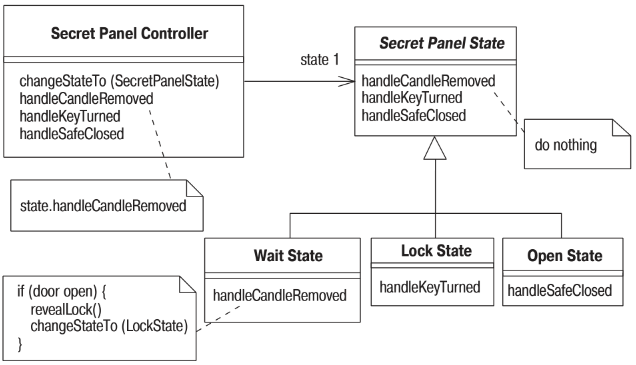
\includegraphics[width=0.5\textwidth]{stateTransitionStatePattern.png}
			\attribution{М. Фаулер, UML. Основы}
		\end{center}
	\end{frame}

	\section{Диаграммы последовательностей}

	\begin{frame}
		\frametitle{Диаграммы последовательностей}
		\begin{columns}
			\begin{column}{0.5\textwidth}
				\begin{itemize}
					\item Применяются для визуализации взаимодействия между объектами
					\begin{itemize}
						\item Особо удобно для асинхронных вызовов
						\item Телекоммуникационные протоколы
					\end{itemize}
					\item Могут применяться на этапе анализа предметной области
					\item Могут применяться для составления плана тестирования
					\item И даже для визуализации логов работающей системы
				\end{itemize}
			\end{column}
			\begin{column}{0.5\textwidth}
				\begin{center}
					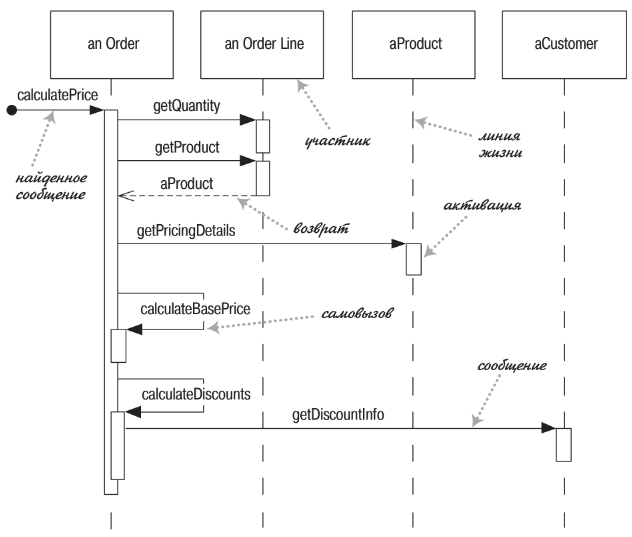
\includegraphics[width=0.9\textwidth]{sequenceDiagramSyntax.png}
					\attribution{М. Фаулер, UML. Основы}
				\end{center}
			\end{column}
		\end{columns}
	\end{frame}

	\begin{frame}
		\frametitle{Ещё немного о синтаксисе}
		\begin{center}
			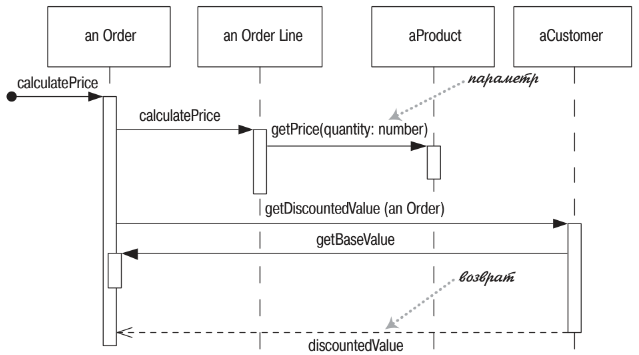
\includegraphics[width=0.6\textwidth]{sequenceDiagramSyntax2.png}
			\attribution{М. Фаулер, UML. Основы}
		\end{center}
	\end{frame}

	\begin{frame}
		\frametitle{Пример}
		\begin{center}
			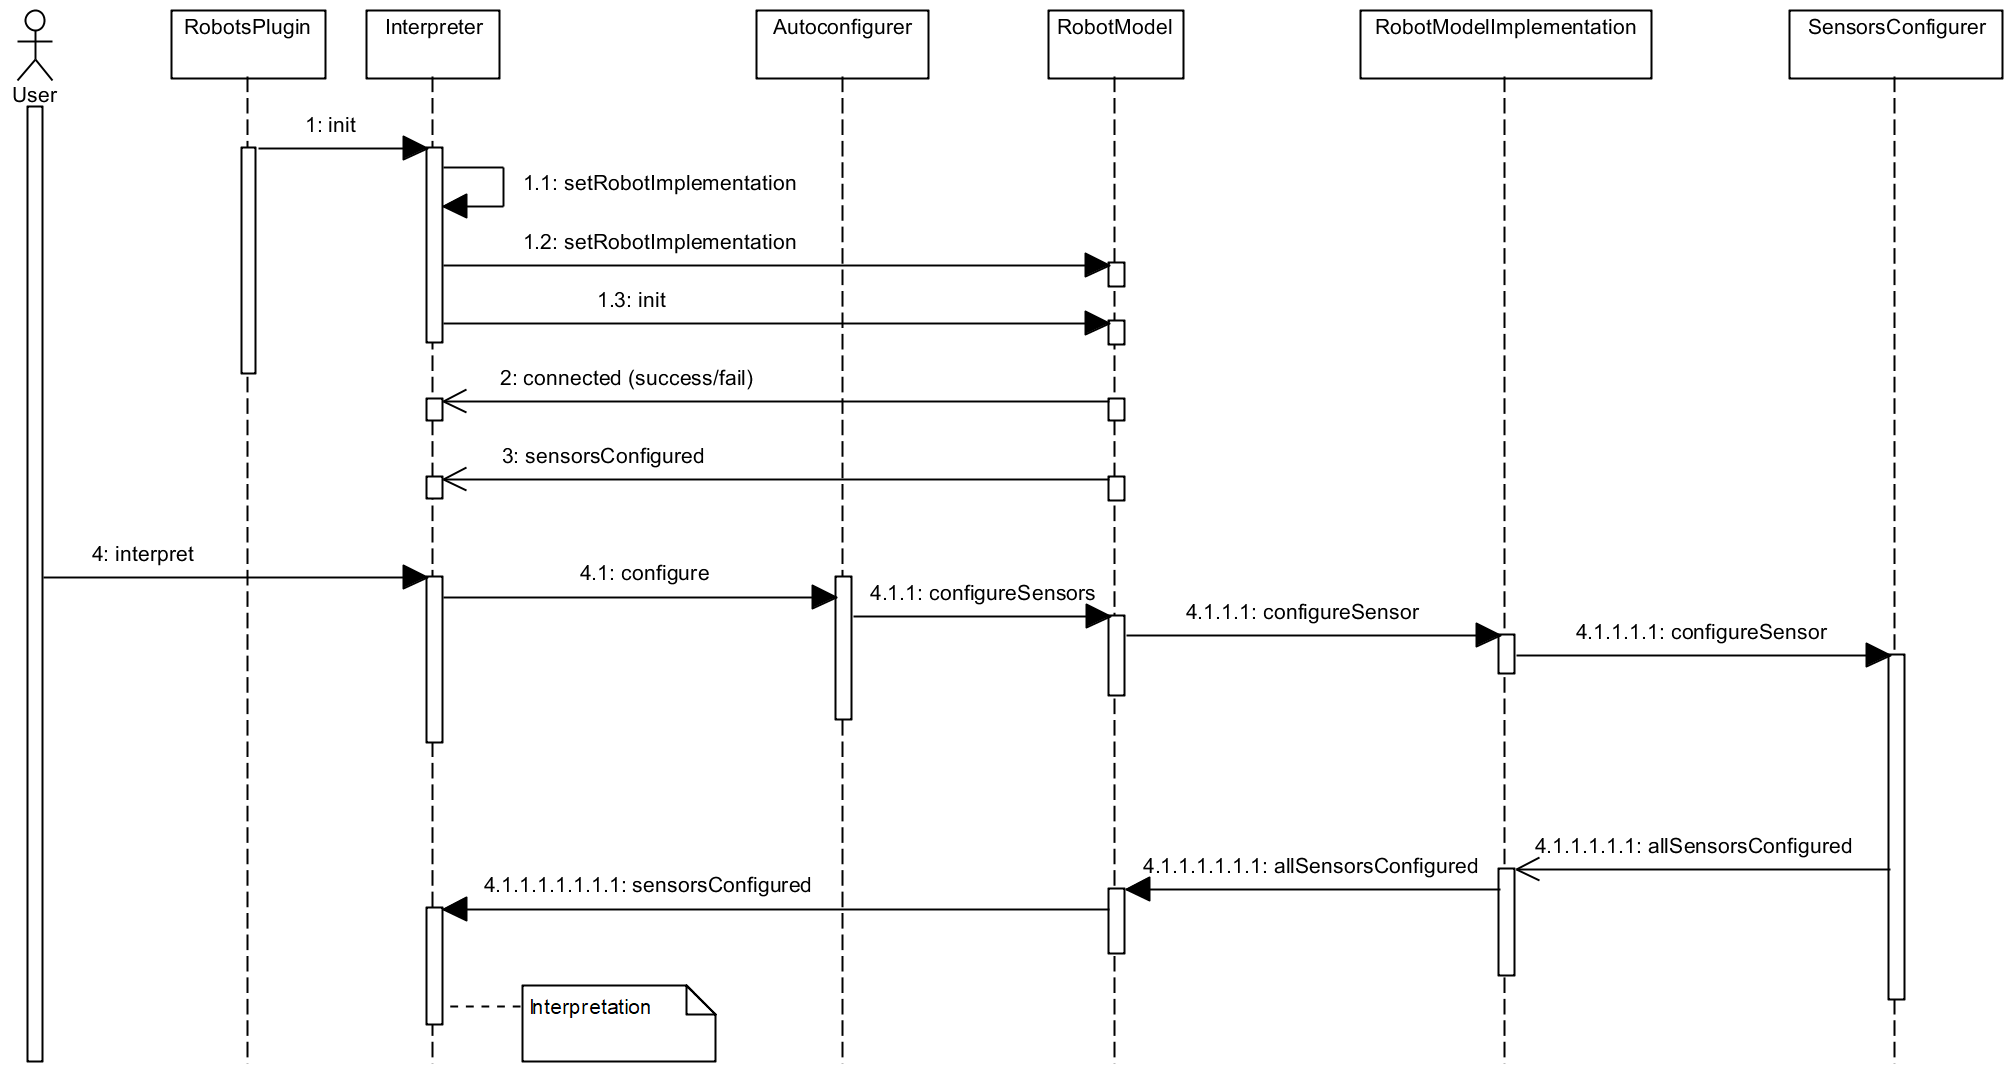
\includegraphics[width=\textwidth]{sequenceDiagramExample.png}
		\end{center}
	\end{frame}

	\begin{frame}
		\frametitle{Ещё пример}
		\begin{center}
			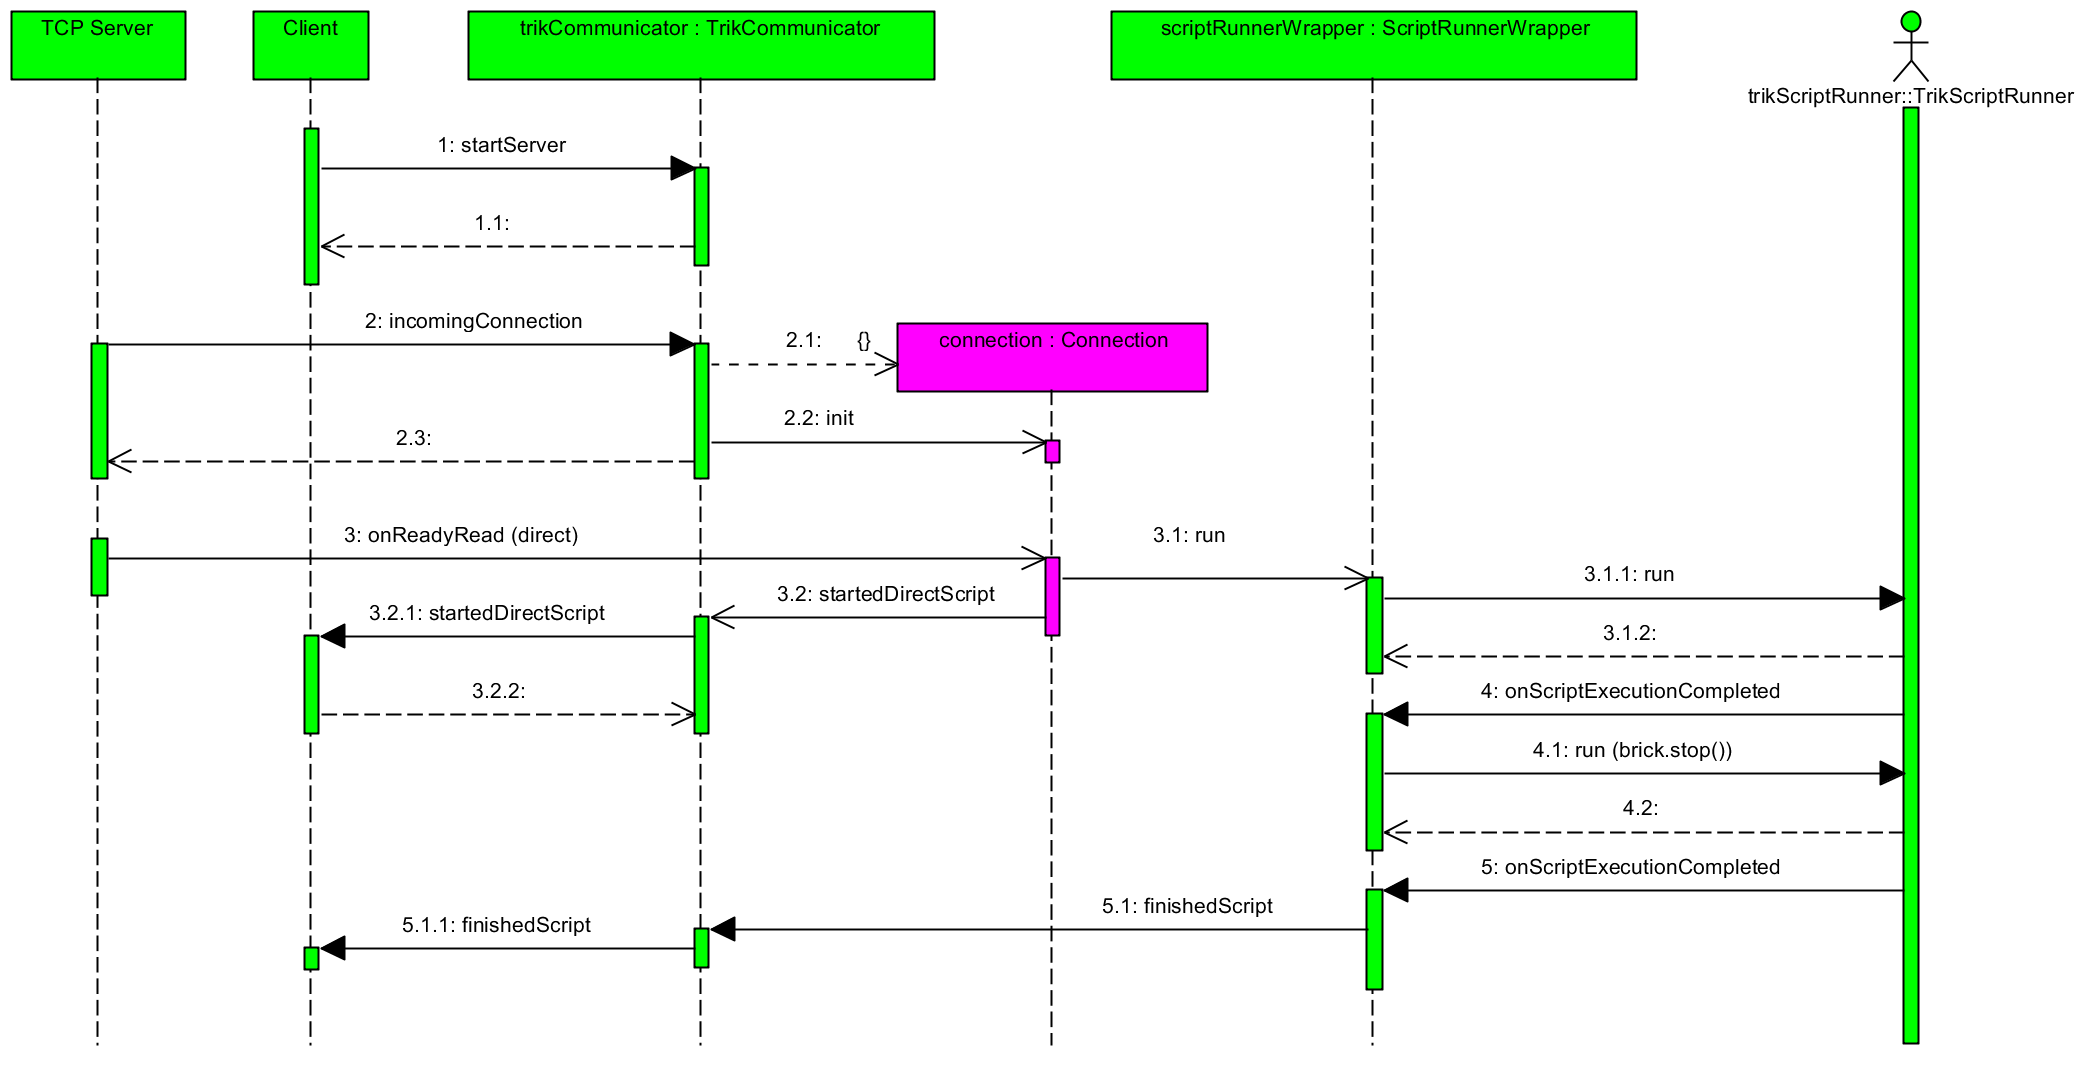
\includegraphics[width=\textwidth]{sequenceDiagramExample2.png}
		\end{center}
	\end{frame}

	\begin{frame}
		\frametitle{И ещё пример}
		\begin{center}
			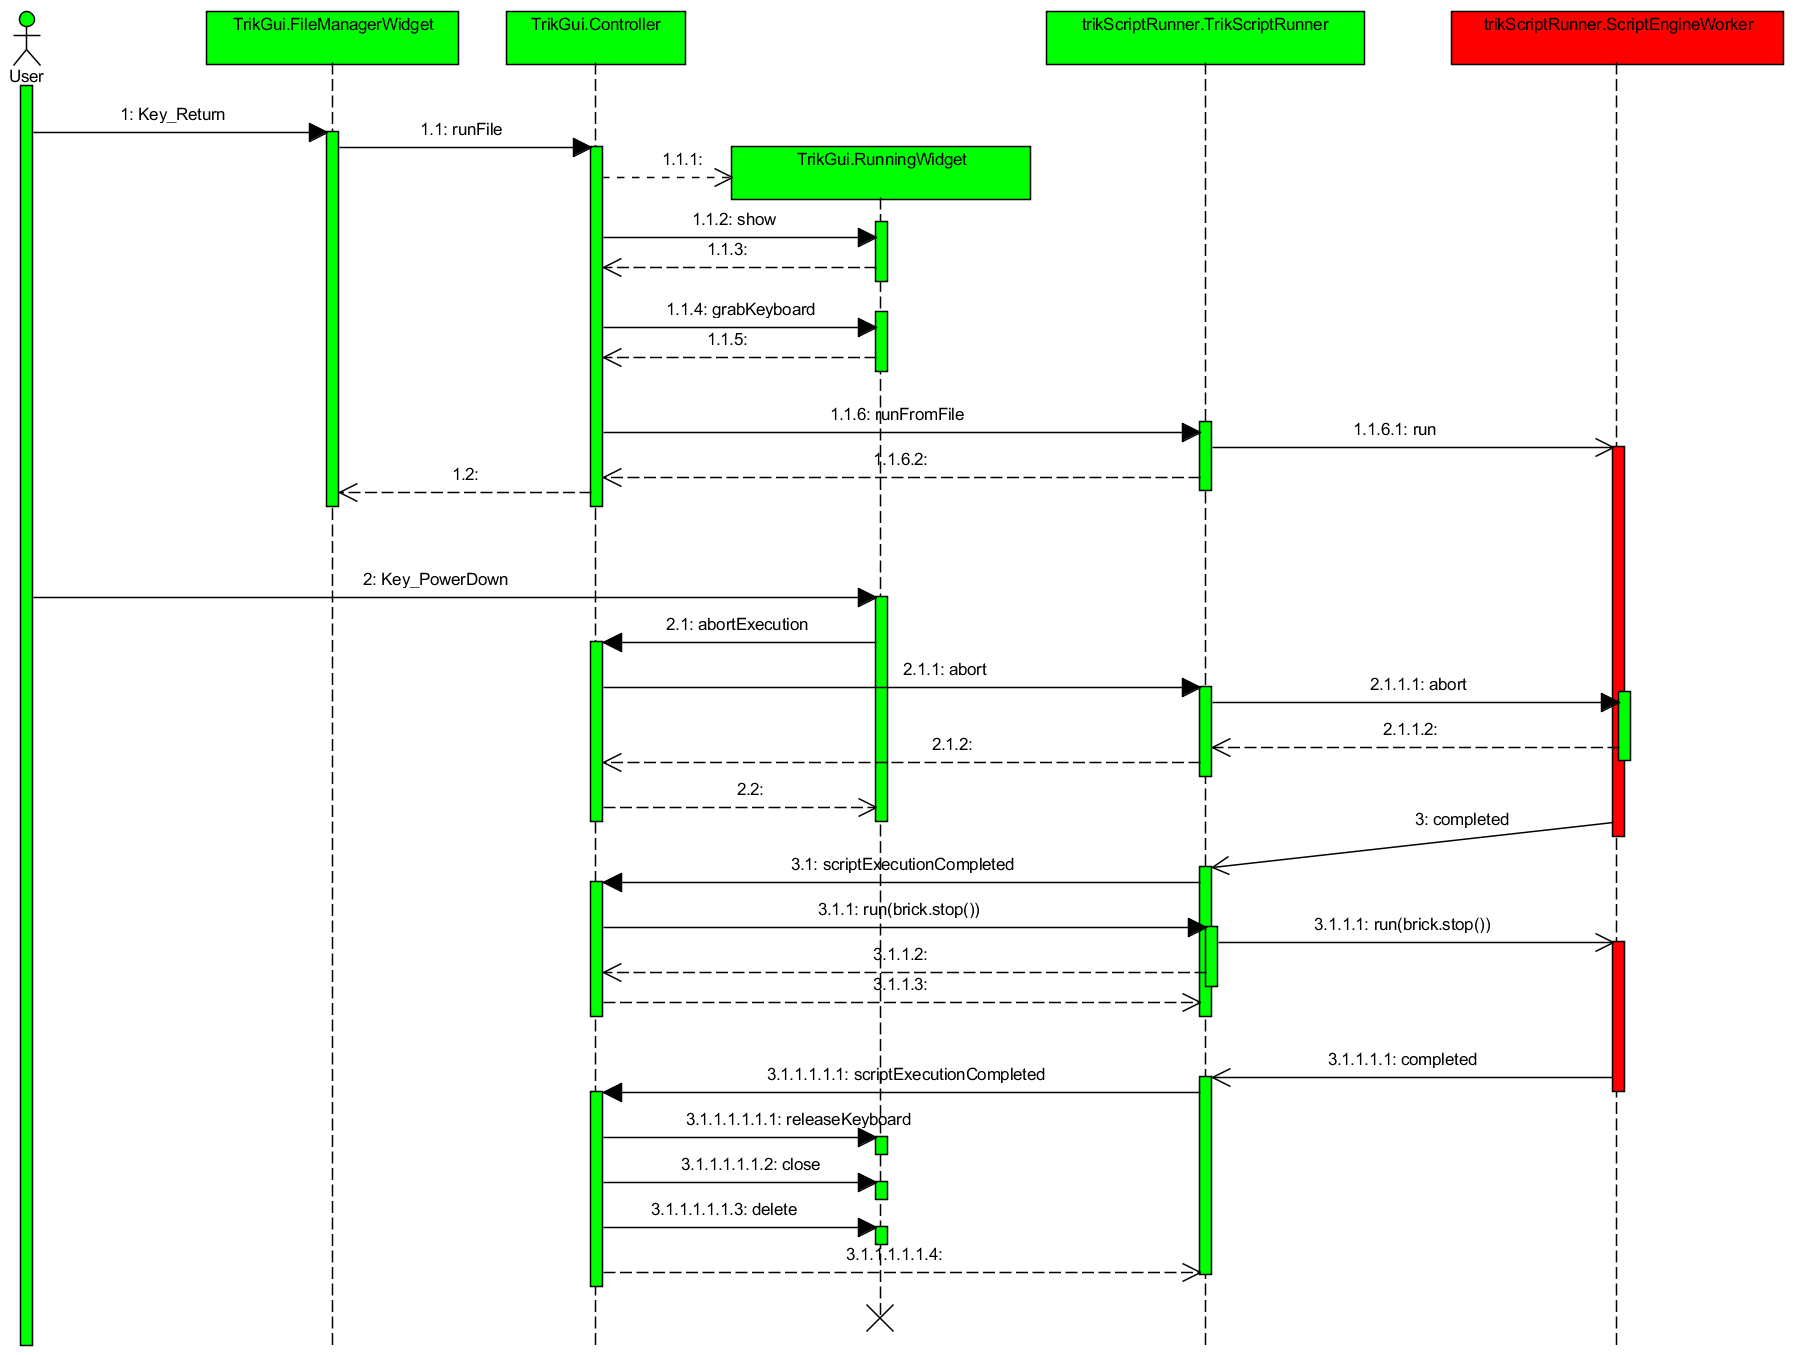
\includegraphics[width=0.8\textwidth]{sequenceDiagramExample3.png}
		\end{center}
	\end{frame}

	\begin{frame}
		\frametitle{Создание и удаление объектов}
		\begin{center}
			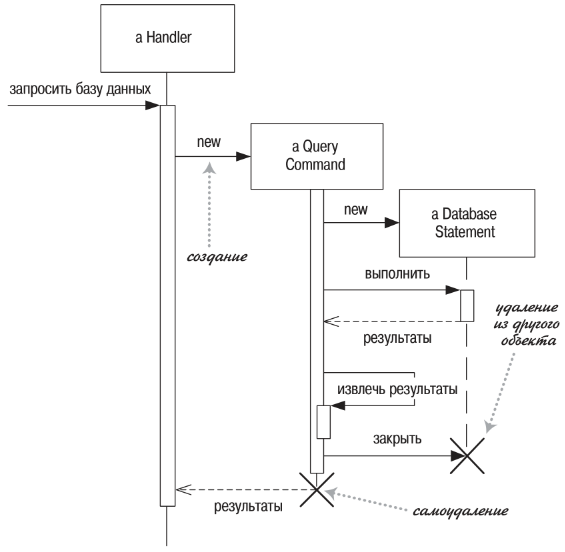
\includegraphics[width=0.5\textwidth]{sequenceDiagramCreationAndDeletion.png}
			\attribution{М. Фаулер, UML. Основы}
		\end{center}
	\end{frame}

	\begin{frame}[fragile]
		\frametitle{Фреймы}
		\begin{columns}
			\begin{column}{0.5\textwidth}
				\begin{small}
					\begin{minted}{text}
    foreach (lineitem)
        if (product.value > $10K)
            careful.dispatch
        else
            regular.dispatch
        end if
    end for
    if (needsConfirmation) 
        messenger.confirm
					\end{minted}
				\end{small}
			\end{column}
			\begin{column}{0.5\textwidth}
				\begin{center}
					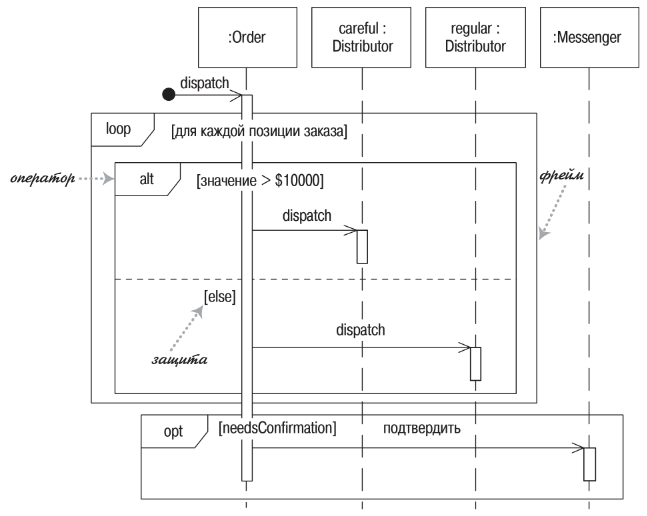
\includegraphics[width=\textwidth]{sequenceDiagramFrames.png}
					\attribution{М. Фаулер, UML. Основы}
				\end{center}
			\end{column}
		\end{columns}
	\end{frame}

	\section{Коммуникационные диаграммы}

	\begin{frame}
		\frametitle{Коммуникационные диаграммы}
		\begin{columns}
			\begin{column}{0.5\textwidth}
				\begin{itemize}
					\item Применяются для визуализации взаимодействия между объектами
					\begin{itemize}
						\item Более легковесный аналог диаграмм последовательностей
						\item Тоже отображают один сценарий взаимодействия
					\end{itemize}
				\end{itemize}
			\end{column}
			\begin{column}{0.5\textwidth}
				\begin{center}
					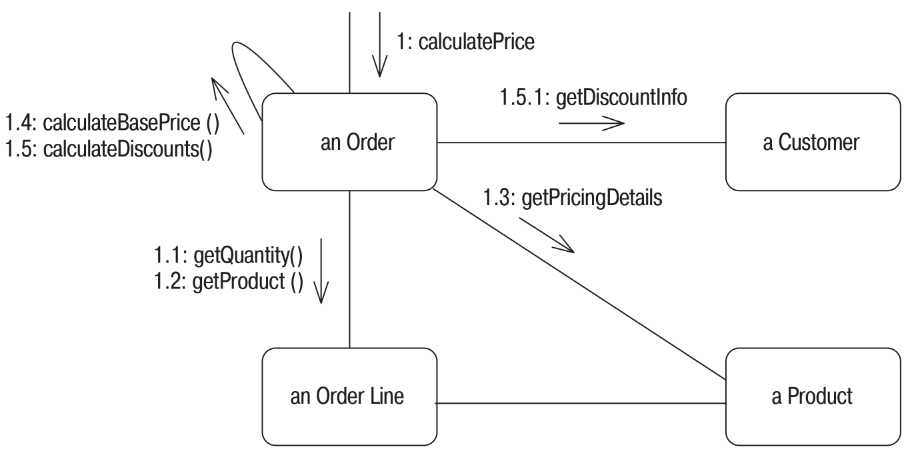
\includegraphics[width=\textwidth]{communicationDiagram.png}
					\attribution{М. Фаулер, UML. Основы}
				\end{center}
			\end{column}
		\end{columns}
	\end{frame}

	\begin{frame}
		\frametitle{Коммуникационные диаграммы, пример}
		\begin{center}
			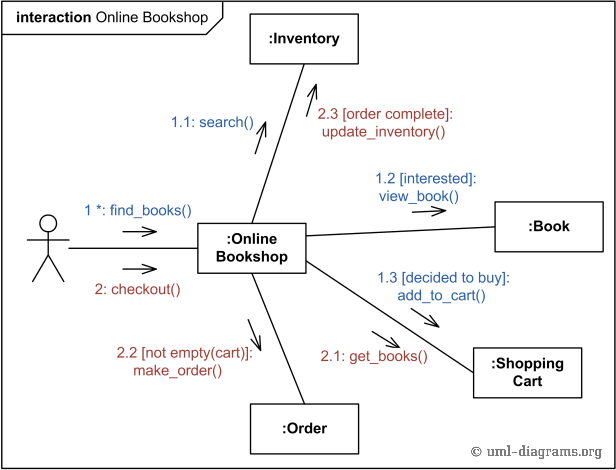
\includegraphics[width=0.6\textwidth]{communicationDiagramExample.png}
			\attribution{http://www.uml-diagrams.org/}
		\end{center}
	\end{frame}

	\section{Диаграммы составных структур}

	\begin{frame}
		\frametitle{Диаграммы составных структур}
		\begin{columns}
			\begin{column}{0.5\textwidth}
				\begin{itemize}
					\item По сути, продвинутые диаграммы компонентов
					\item Внутри компоненты не другие компоненты, а части (роли)
				\end{itemize}
				\vspace{3mm}
				\begin{center}
					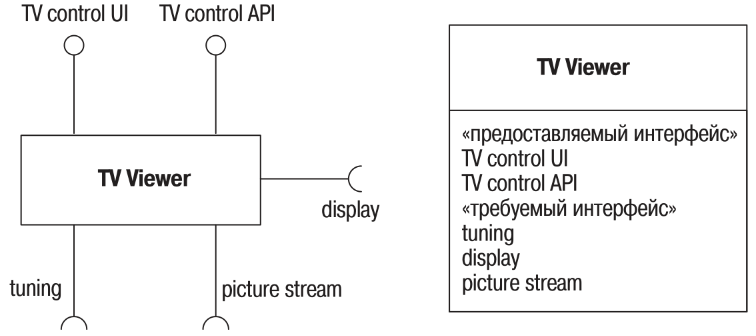
\includegraphics[width=0.9\textwidth]{compositeStructureElement.png}
				\end{center}
			\end{column}
			\begin{column}{0.5\textwidth}
				\begin{center}
					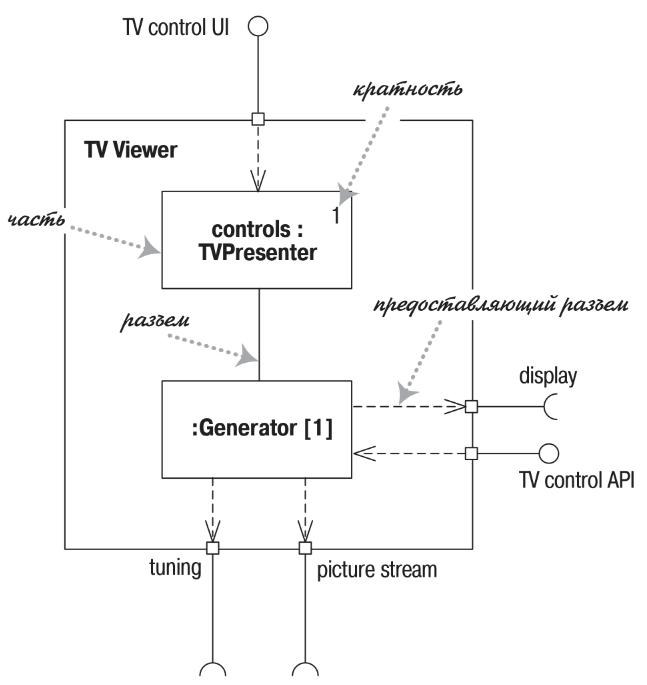
\includegraphics[width=0.8\textwidth]{compositeStructureDiagram.png}
					\attribution{М. Фаулер, UML. Основы}
				\end{center}
			\end{column}
		\end{columns}
	\end{frame}

	\begin{frame}
		\frametitle{Диаграммы составных структур, пример}
		\begin{center}
			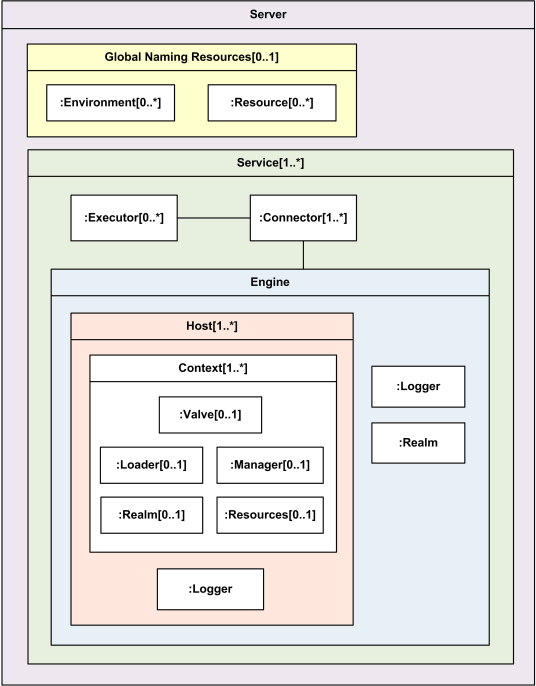
\includegraphics[width=0.45\textwidth]{compositeStructureExample.png}
			\attribution{http://www.uml-diagrams.org/}
		\end{center}
	\end{frame}

	\section{Диаграммы коопераций}

	\begin{frame}
		\frametitle{Диаграммы коопераций}
		\begin{columns}
			\begin{column}{0.5\textwidth}
				\begin{itemize}
					\item Показывают взаимодействие между объектами (ролями) в рамках одного сценария использования
				\end{itemize}
				\vspace{3mm}
				\begin{center}
					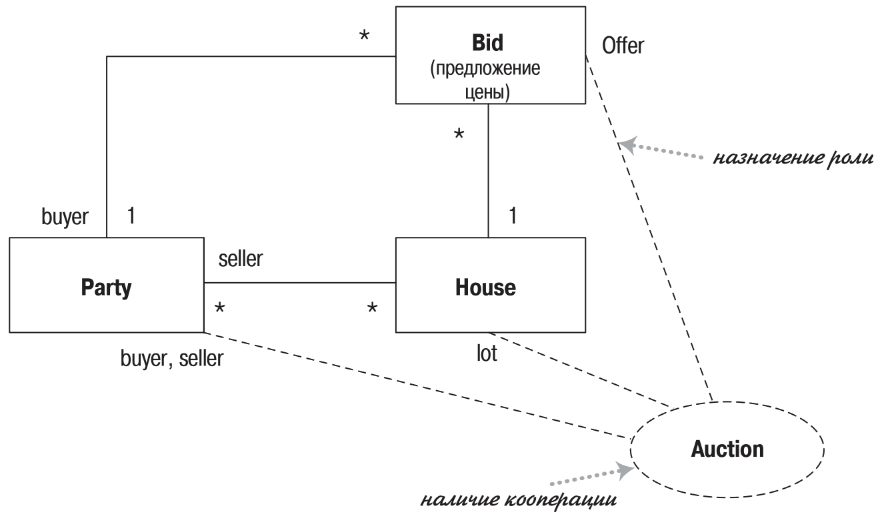
\includegraphics[width=0.9\textwidth]{cooperationAlternateNotation.png}
				\end{center}
			\end{column}
			\begin{column}{0.5\textwidth}
				\begin{center}
					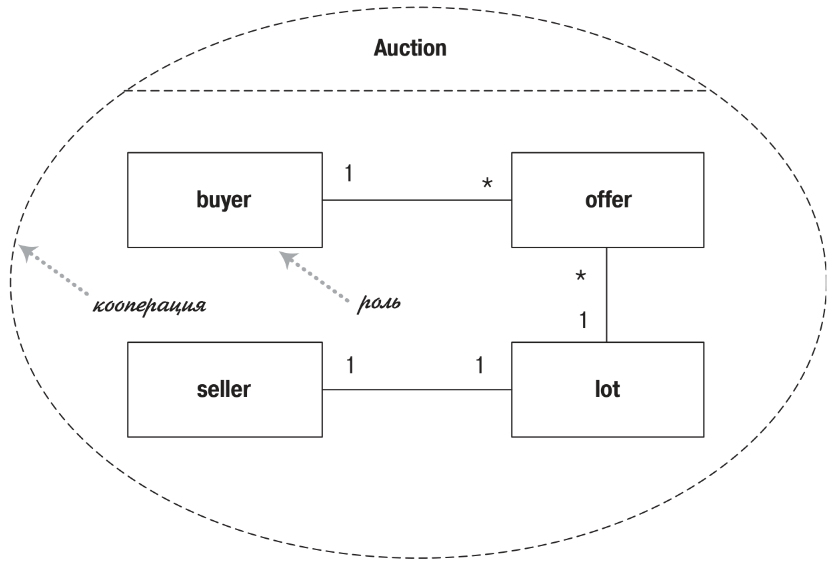
\includegraphics[width=0.9\textwidth]{cooperationDiagram.png}
					\attribution{М. Фаулер, UML. Основы}
				\end{center}
			\end{column}
		\end{columns}
	\end{frame}

	\begin{frame}
		\frametitle{Диаграммы коопераций, последовательности}
		\begin{columns}
			\begin{column}{0.5\textwidth}
				\begin{center}
					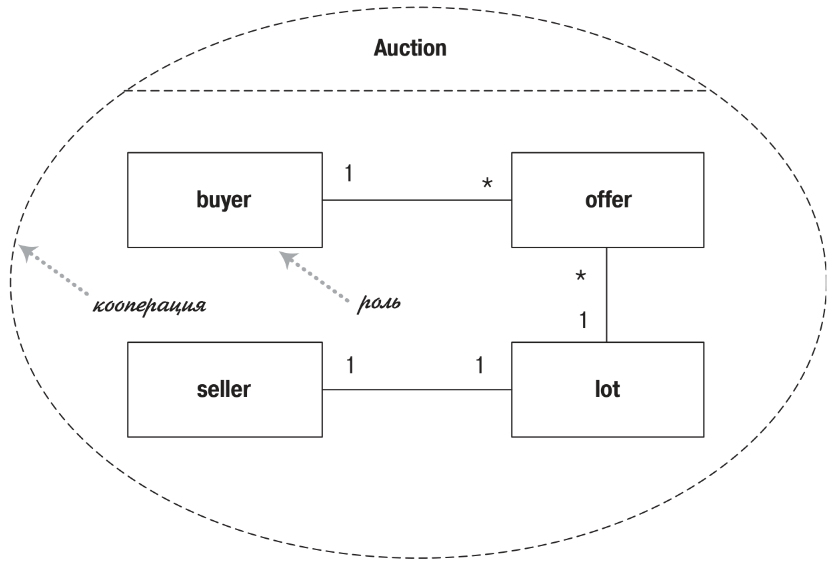
\includegraphics[width=0.9\textwidth]{cooperationDiagram.png}
				\end{center}
			\end{column}
			\begin{column}{0.5\textwidth}
				\begin{center}
					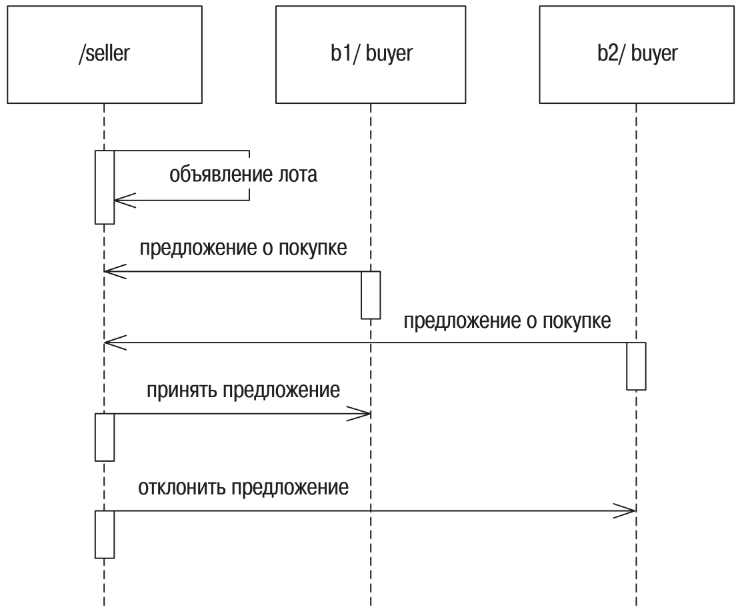
\includegraphics[width=0.9\textwidth]{cooperationSequenceDiagram.png}
					\attribution{М. Фаулер, UML. Основы}
				\end{center}
			\end{column}
		\end{columns}
	\end{frame}

	\section{Временные диаграммы}

	\begin{frame}
		\frametitle{Временные диаграммы}
		\begin{columns}
			\begin{column}{0.5\textwidth}
				\begin{itemize}
					\item Для моделирования временных ограничений в системах реального времени
				\end{itemize}
				\vspace{3mm}
				\begin{center}
					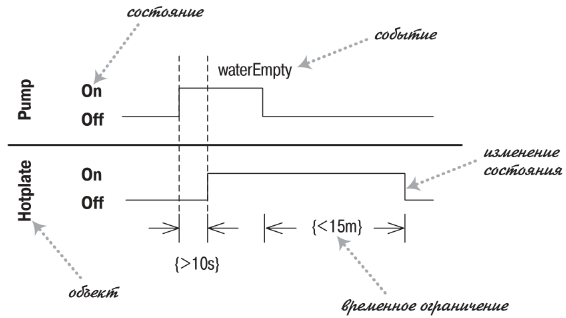
\includegraphics[width=0.9\textwidth]{timingDiagrams.png}
				\end{center}
			\end{column}
			\begin{column}{0.5\textwidth}
				\begin{center}
					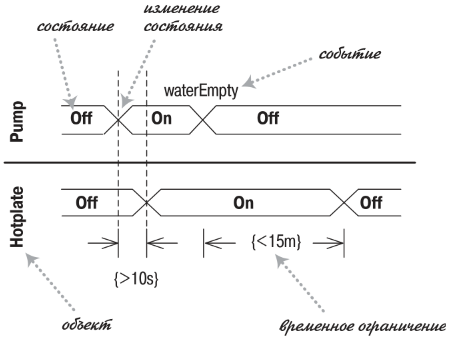
\includegraphics[width=0.8\textwidth]{timingDiagramsAlternate.png}
					\attribution{М. Фаулер, UML. Основы}
				\end{center}
			\end{column}
		\end{columns}
	\end{frame}

	\begin{frame}
		\frametitle{Временная диаграмма, пример}
		\begin{center}
			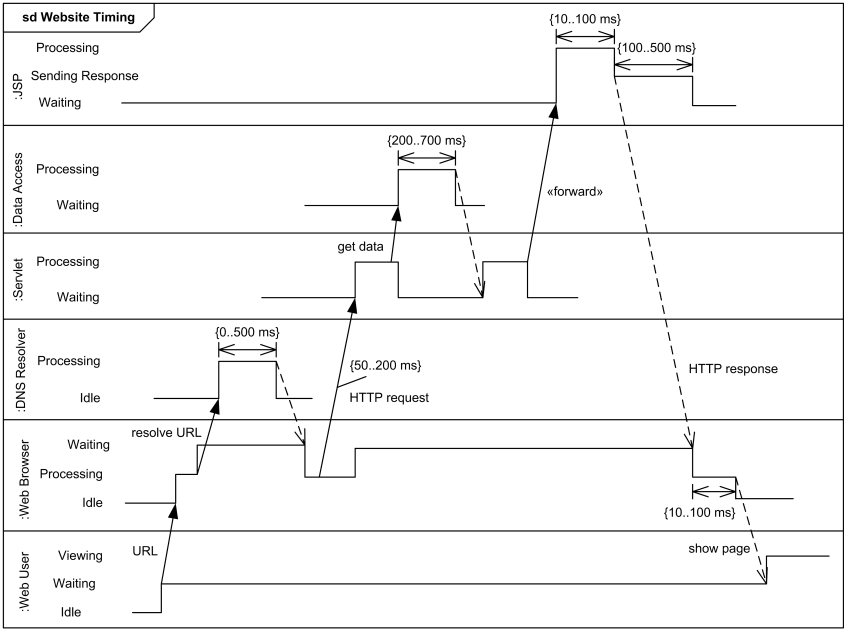
\includegraphics[width=0.7\textwidth]{timingDiagramExample.png}
			\attribution{http://www.uml-diagrams.org/}
		\end{center}
	\end{frame}

	\section{Диаграммы обзора взаимодействия}

	\begin{frame}
		\frametitle{Диаграммы обзора взаимодействия}
		\begin{columns}
			\begin{column}{0.5\textwidth}
				\begin{itemize}
					\item Диаграммы активностей + диаграммы последовательностей
					\item Применяются при наличии взаимодействия со сложной логикой, когда фреймы неудобны
				\end{itemize}
			\end{column}
			\begin{column}{0.5\textwidth}
				\begin{center}
					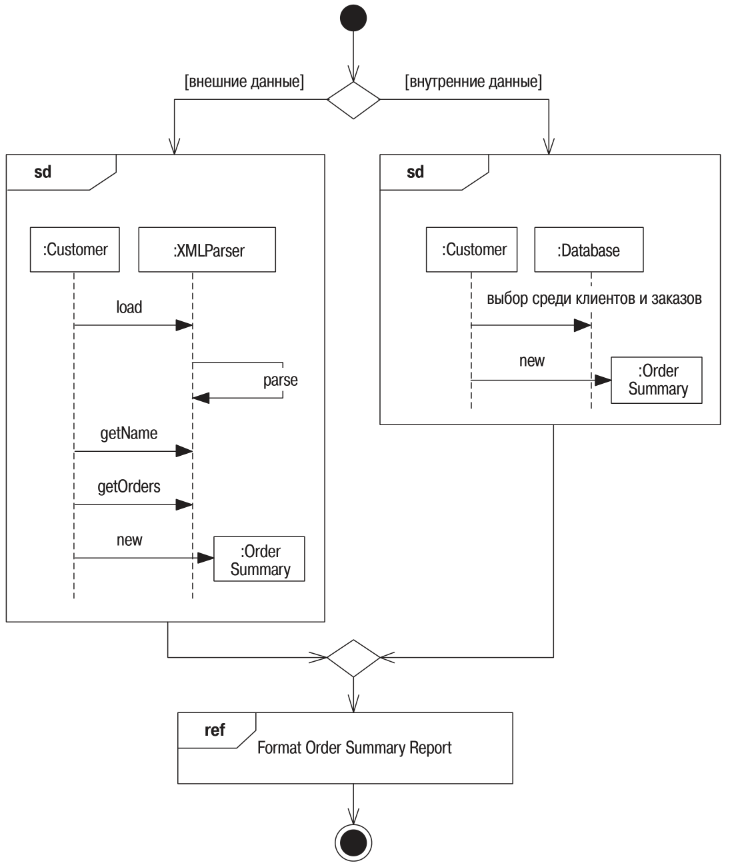
\includegraphics[width=0.9\textwidth]{interactionOverviewDiagrams.png}
					\attribution{М. Фаулер, UML. Основы}
				\end{center}
			\end{column}
		\end{columns}
	\end{frame}

	\begin{frame}
		\frametitle{Диаграмма обзора взаимодействия, пример}
		\begin{center}
			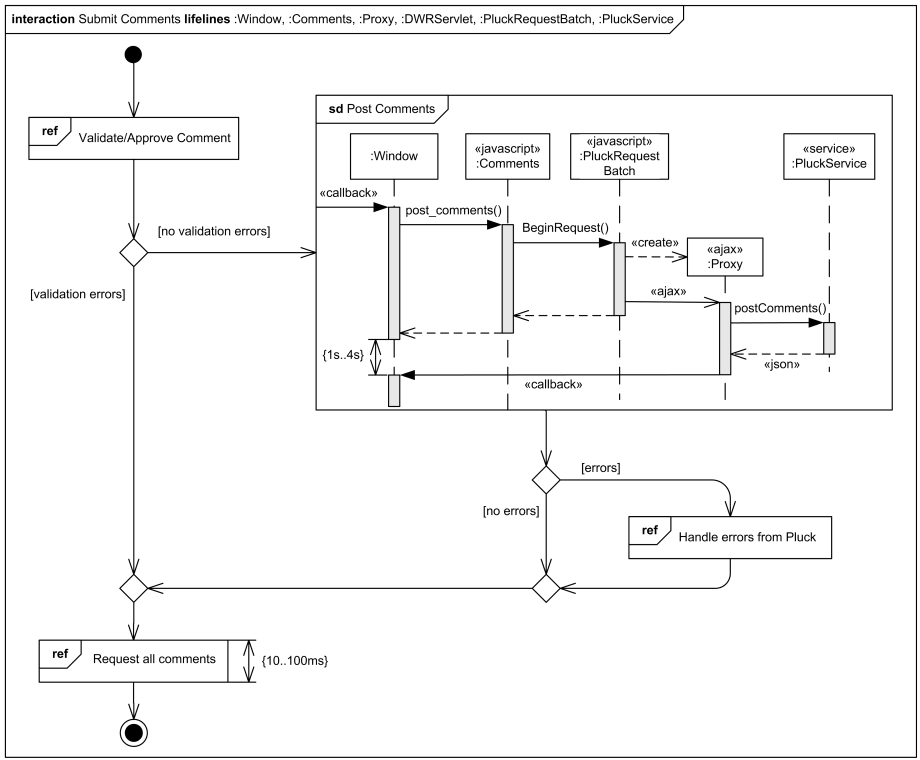
\includegraphics[width=0.7\textwidth]{interactionOverviewExample.png}
			\attribution{http://www.uml-diagrams.org/}
		\end{center}
	\end{frame}

	\section{Заключение}

	\begin{frame}
		\frametitle{Книжка}
		\begin{columns}
			\begin{column}{0.5\textwidth}
				\begin{center}
					
\includegraphics[width=0.4\textwidth]{umlBookCover.png}
				\end{center}
			\end{column}
			\begin{column}{0.5\textwidth}
				М. Фаулер, UML. Основы. Краткое руководство по стандартному языку объектного моделирования. СПб., Символ-Плюс, 2011. 192 С.
			\end{column}
		\end{columns}
	\end{frame}

	\section{Домашнее задание}

	\begin{frame}
		\frametitle{Домашнее задание, вариант 1}
		\begin{small}
			\begin{enumerate}
				\item Нарисуйте с помощью диаграмм классов UML следующий фрагмент предметной области. Вот
					перечень учреждений, которые могут выдавать общегражданские загранпаспорта в РФ: в
					пределах РФ --- органы МВД по месту жительства; МИД РФ и его представительствами на
					территории РФ; вне пределов РФ --- дипломатическими представительствами или
					консульскими учреждениями РФ.
				\item Нарисуйте с помощью диаграмм классов UML следующий фрагмент предметной области. Есть
					лес, в нем растут деревья --- сосны, березы, ивы. Березы бывают следующих видов: береза
					бумажная, береза вишневая, береза даурская. Сосны бывают следующих видов: сосна
					чешуйчатая, сосна уэмацу, сосна юньнаньская. У каждого дерева есть ствол, ветви, коневая
					система. Еще в лесу живут птицы --- синицы, дрозды, совы (ушастая и болотная).
				\item Нарисуйте с помощью диаграмм классов UML следующий фрагмент предметной области.
					<<Учебный курс в университете>>.
			\end{enumerate}
		\end{small}
	\end{frame}

	\begin{frame}
		\frametitle{Домашнее задание, вариант 2}
		\begin{small}
			\begin{enumerate}
				\item Нарисуйте с помощью диаграмм классов UML следующий фрагмент предметной области.
					Органы власти в России подразделяются на государственные и муниципальные.
					Государственные органы власти бывают центральными и региональными, а также субъектов
					федерации. Субъекты бывают следующих видов --- республики, края, области, города
					федерального значения, автономная область и автономные округа.
				\item Нарисуйте с помощью диаграмм классов UML следующий фрагмент предметной области.
					Общегражданский загранпаспорт РФ бывает следующих видов --- обычный и нового
					поколения. Владельцами загранпаспорта могут быть дети и взрослые (владельцы агрегируют
					свои загранпаспорта). Другими видами документов для выезда из РФ являются
					дипломатический паспорт, служебный паспорт, паспорт моряка.
				\item Нарисуйте с помощью диаграмм классов UML фрагмент предметной области. <<Сдача
					экзамена>>.
			\end{enumerate}
		\end{small}
	\end{frame}

	\begin{frame}
		\frametitle{Домашнее задание, вариант 3}
		\begin{small}
			\begin{enumerate}
				\item Нарисуйте с помощью диаграмм классов UML следующий фрагмент предметной области.
					Деревья в лесу бывают следующих видов --- сосны, березы, ивы. Березы бывают следующих
					видов: береза бумажная, береза вишневая, береза даурская. Сосны бывают следующих
					видов: сосна чешуйчатая, сосна уэмацу, сосна юньнаньская.
				\item Нарисуйте с помощью диаграмм классов UML следующий фрагмент предметной области. Банк
					состоит из различных филиалов, а также головного офиса. Все подразделения банка состоят
					из департаментов. Департаменты бывают производственными и административными. В
					департаментах работают сотрудники.
				\item Нарисуйте с помощью диаграмм классов UML фрагмент предметной области <<Поселение в
					общежитие>>.
			\end{enumerate}
		\end{small}
	\end{frame}

\end{document}